% !TEX program = xelatex
% c5p-s-2026-final.tex
% 2026 €€£ 超专业级别硬件能力认证第一轮（C5P-S1）提高级 C++语言试题（模拟卷）
% 版式：a4paper、等线题头、宋体中文 + Consolas 西文、页脚两行（PDF 格式）、选项每行一个、大题强制换页
% 代码：带边框、左侧行号 0 补齐、无横向线条；阅读程序不写概要，完善程序写概要后挖空
% 编译方式：xelatex c5p-s-2026-final.tex（建议编译两次）
\documentclass[a4paper]{ctexart}

\usepackage{fontspec}
\usepackage{graphicx}
\usepackage{tikz}
\usetikzlibrary{arrows.meta}
\usepackage{eso-pic}
\newcommand{\waterword}{%
  \makebox[0pt][c]{%
    \tikz[baseline]{%
      \node[
        inner sep=0pt,
        rotate=-35,
        text=black,
        opacity=0.085,
        font=\fontsize{54}{70}\selectfont
      ] {折工};%
    }%
  }%
}
\AddToShipoutPictureFG{%
  \put(\LenToUnit{-0.3cm},\LenToUnit{1.2cm}){\waterword}%
  \put(\LenToUnit{5.0cm},\LenToUnit{0.0cm}){\waterword}%
  \put(\LenToUnit{10.3cm},\LenToUnit{1.4cm}){\waterword}%
  \put(\LenToUnit{15.6cm},\LenToUnit{0.2cm}){\waterword}%
  \put(\LenToUnit{2.2cm},\LenToUnit{6.2cm}){\waterword}%
  \put(\LenToUnit{7.5cm},\LenToUnit{4.8cm}){\waterword}%
  \put(\LenToUnit{12.8cm},\LenToUnit{6.3cm}){\waterword}%
  \put(\LenToUnit{18.1cm},\LenToUnit{4.9cm}){\waterword}%
  \put(\LenToUnit{-0.3cm},\LenToUnit{10.0cm}){\waterword}%
  \put(\LenToUnit{5.0cm},\LenToUnit{11.5cm}){\waterword}%
  \put(\LenToUnit{10.3cm},\LenToUnit{10.1cm}){\waterword}%
  \put(\LenToUnit{15.6cm},\LenToUnit{11.6cm}){\waterword}%
  \put(\LenToUnit{2.2cm},\LenToUnit{16.5cm}){\waterword}%
  \put(\LenToUnit{7.5cm},\LenToUnit{15.1cm}){\waterword}%
  \put(\LenToUnit{12.8cm},\LenToUnit{16.6cm}){\waterword}%
  \put(\LenToUnit{18.1cm},\LenToUnit{15.2cm}){\waterword}%
  \put(\LenToUnit{-0.3cm},\LenToUnit{21.6cm}){\waterword}%
  \put(\LenToUnit{5.0cm},\LenToUnit{23.1cm}){\waterword}%
  \put(\LenToUnit{10.3cm},\LenToUnit{21.7cm}){\waterword}%
  \put(\LenToUnit{15.6cm},\LenToUnit{23.2cm}){\waterword}%
  \put(\LenToUnit{2.2cm},\LenToUnit{27.3cm}){\waterword}%
  \put(\LenToUnit{7.5cm},\LenToUnit{25.9cm}){\waterword}%
  \put(\LenToUnit{12.8cm},\LenToUnit{27.4cm}){\waterword}%
  \put(\LenToUnit{18.1cm},\LenToUnit{26.0cm}){\waterword}%
}
\usepackage{geometry}
\geometry{top=2.7cm, left=2.7cm, right=2.7cm, bottom=4cm}
\setmainfont{Consolas}
\setmonofont{Consolas}
\setCJKmainfont{SimSun}
\newCJKfontfamily{\dengxian}{DengXian}

\usepackage{fancyhdr}
\usepackage{lastpage}
\usepackage[most]{tcolorbox}
\usepackage{listings}
\usepackage{enumitem}
\usepackage{amsmath}
\usepackage{xcolor}
\DeclareMathSizes{10.53937}{10.95}{7.5}{5.5}

% 将带圈数字 ①-⑤ 划入 CJK 字符类，确保题干“①处应填”用中文字体正常渲染
\xeCJKDeclareCharClass{CJK}{"2460 -> "2464}

% ---------------- 页脚：中文宋体 + 数字英文 Times New Roman（参考 cspjs2024hs.pdf 样式） ----------------
\newfontfamily\trm{Times New Roman}
% 普通 Unicode 黑圆点，避免依赖 Wingdings 私有字形映射
\newcommand{\wdot}{{\fontsize{12}{12}\selectfont\textbullet}}
\pagestyle{fancy}
\fancyhf{}
\setlength{\footskip}{1.5cm}
\fancyfoot[C]{{\xeCJKsetup{CJKecglue={\hskip0pt}}{\trm €€£ C5P-S 2026 }{\songti 第一轮 }{\trm C++}{\songti 语言试题}}\\[2pt]{\xeCJKsetup{CJKecglue={\hskip0pt}}{\songti 第}{\trm\thepage}{\songti 页，共}{\trm\pageref{LastPage}}{\songti 页}}}
\renewcommand{\headrulewidth}{0pt}
\renewcommand{\footrulewidth}{0pt}

% ---------------- 代码样式：框宽 14cm、Consolas 12pt、行号 8.5pt(约0.3cm高)、关键字不加粗 ----------------
\renewcommand{\thelstnumber}{\ifnum\value{lstnumber}<10 0\fi\arabic{lstnumber}}
\lstset{
  language=C++,
  basicstyle=\ttfamily\fontsize{12}{14.4}\selectfont,
  numberstyle=\ttfamily\fontsize{12}{14.4}\selectfont\makebox[0.92cm][r],
  numbers=left,
  firstnumber=1,
  stepnumber=1,
  numberfirstline=true,
  numbersep=0.08cm,
  frame=none,
  framesep=6pt,
  rulecolor=\color{black!70},
  columns=fullflexible,
  keepspaces=true,
  aboveskip=0pt,
  belowskip=0pt,
  xleftmargin=0.88cm,
  linewidth=14.55cm,
  showstringspaces=false,
  breaklines=true,
  breakatwhitespace=false,
  keywordstyle=\ttfamily,
  commentstyle=\ttfamily,
  stringstyle=\ttfamily,
  escapeinside={|@}{@|},
}

% 代码框：线1（左框线）距页左 2.05cm；行号列线1→线2 严格 1cm；代码列线2→线3 严格 14.55cm；
% 线3（右框线）距页右约 3.40cm（A4 宽 21cm 自动吻合）；挖空下划线 2.10cm + 居中序号
\newtcolorbox{codebox}{enhanced, breakable, sharp corners, boxrule=0.5pt, colframe=black, colback=white,
  width=15.0cm, left skip=-0.65cm, before skip=6pt, after skip=8pt,
  top=2pt, bottom=2pt, left=0pt, right=0pt,
  overlay={\draw[black,line width=0.5pt] ([xshift=1.0cm]frame.north west)--([xshift=1.0cm]frame.south west);}}
% 完善程序挖空：2.10cm 下划线 + 居中序号（字体同代码 12pt）
\newcommand{\blank}[1]{\underline{\makebox[2.1cm][c]{#1}}}

\setlength{\parindent}{0pt}
\setlength{\parskip}{2pt}
\linespread{1.25}

% 大题标题（左对齐黑体）
\newcommand{\bigtitle}[1]{\noindent\heiti #1\par\vspace{2pt}}
% 小题题干（序号数字不加粗，Consolas）
\newcommand{\q}[1]{\noindent #1}
% 阅读程序小题：题号前加 Unicode 黑点（整体左对齐）
\newcommand{\qdot}[1]{\noindent\wdot\hspace{0.6em}#1}
% 单个选项（每个选项独立一行）
\newcommand{\opt}[1]{\hspace*{2em} #1\par}
% 完善程序选项：两个选项一行（A B 一行、C D 一行）
\newcommand{\optw}[2]{\hspace*{2em} #1\hspace*{2em}#2\par}

\begin{document}

\begin{center}
{\dengxian
{\xeCJKsetup{CJKecglue={\hskip 0.419em}}\fontsize{15.95}{1}\selectfont 2026 €€£超专业级别硬件能力认证第一轮} \\[1.5em]
    {\xeCJKsetup{CJKecglue={\hskip 0.419em}}\fontsize{15.95}{1}\selectfont （C5P-S1） 提高级 C++\hspace{0pt}语言试题} \\[1.5em]
{\xeCJKsetup{CJKecglue={\hskip 0.344em}}\fontsize{14.05}{1}\selectfont 认证时间：2026年9月18日14:30\textasciitilde16:30}\\[1em]
{\fontsize{12}{1}\selectfont 编者：唐一潇、季灵、裘泽燑}
}
\end{center}

\vspace{8pt}
\noindent{\heiti 考生注意事项：}
\begin{itemize}[leftmargin=2.6em, itemsep=1pt, label={}]
  \item \wdot\hspace{0.5em}试题纸共有 \pageref{LastPage} 页，答题纸共有 1 页，满分 100 分。请在答题纸上作答，写在试题纸上的一律无效。
    \item \wdot\hspace{0.5em}不得使用任何电子设备（如计算器、手机、电子词典等）或查阅任何书籍资料。
\end{itemize}

\bigtitle{一、单项选择题（共 15 题，每题 2 分，共计 30 分；每题有且仅有一个正确选项）}
\q{1.} 下列 Linux 命令中，用于连接并显示文件内容的是（\qquad）\\
\opt{A. \texttt{cp}}\opt{B. \texttt{cat}}\opt{C. \texttt{ping}}\opt{D. \texttt{touch}}
\q{2.} 已知某用二叉链表存储的哈夫曼树共有 \texttt{m} 个叶子结点，则该哈夫曼树中总共有多少个空指针域（\qquad）\\
\opt{A. \texttt{m}}\opt{B. \texttt{m+1}}\opt{C. \texttt{2m}}\opt{D. \texttt{2m+1}}
\q{3.} 对于一棵高度为 \texttt{h} 的完全 5 叉树，对每个叶子结点向上访问直到根结点，统计路径上经过的结点数之和。总时间复杂度为（\qquad）\\
\opt{A. \(\Theta(5^h)\)}\opt{B. \(\Theta(h5^h)\)}\opt{C. \(\Theta(5h)\)}\opt{D. \(\Theta(h^2)\)}
\q{4.} 小 h 从原点 \texttt{(0,0)} 出发，每一步向右或向上走，到达点 \texttt{(5,5)}，且始终满足 \texttt{x >= y}。满足条件的路径有多少条（\qquad）\\
\opt{A. 252}\opt{B. 90}\opt{C. 132}\opt{D. 42}
\q{5.} 用两个栈模拟一个队列，入队时元素统一压入栈 A。正确的出队操作是（\qquad）\\
\opt{A. B 为空时将 A 全部转移到 B，再从 B 弹出；B 非空时直接从 B 弹出}
\opt{B. 无论 B 是否为空，都先将 A 全部转移到 B，再从 B 弹出}
\opt{C. 直接删除 A 的栈底元素}\opt{D. 直接从 A 弹出栈顶元素}
\q{6.} 从集合 \texttt{\{1,2,3,\ldots,20\}} 中选出 6 个不同的数，要求任意两个被选数都不相邻。不同的选法共有（\qquad）\\
\opt{A. 3003}\opt{B. 3876}\opt{C. 5005}\opt{D. 8008}
\q{7.} 关于 C++ 标准库容器，下列说法正确的是（\qquad）\\
\opt{A. \texttt{vector} 在头部插入或删除元素的复杂度为 \texttt{O(1)}}
\opt{B. \texttt{deque} 支持 \texttt{O(1)} 随机访问，且在两端插入、删除元素的复杂度为 \texttt{O(1)}}
\opt{C. \texttt{set} 允许存储多个键值相同的元素}
\opt{D. \texttt{priority\_queue::top()} 会返回并删除堆顶元素}
\q{8.} 关于有向无环图的拓扑排序，下列说法正确的是（\qquad）\\
\opt{A. 任何有向无环图的拓扑排序都唯一}\opt{B. 含有环的有向图也可以进行拓扑排序}
\opt{C. 若有边 \texttt{u -> v}，则任一拓扑序中 \texttt{u} 在 \texttt{v} 之前}\opt{D. 拓扑排序就是深度优先遍历序列}
\q{9.} 对文本串 \texttt{T=abababababa} 查找模式串 \texttt{P=ababa}，采用记录每个前缀最长相等真前后缀长度的字符串匹配方法，允许匹配重叠。若下标从 0 开始，所有匹配起始位置之和为（\qquad）\\
\opt{A. 8}\opt{B. 10}\opt{C. 12}\opt{D. 14}
\q{10.} 关于最短路算法（包含最坏情况），下列说法正确的是（\qquad）\\
\opt{A. 对没有负环的图，SPFA 的最坏时间复杂度为 \texttt{O(n+m)}}
\opt{B. 边权非负时，使用邻接表和二叉堆的 Dijkstra 算法复杂度为 \texttt{O((n+m) log n)}}
\opt{C. Bellman--Ford 算法不能判断从源点可达的负环}
\opt{D. Floyd--Warshall 算法的时间复杂度为 \texttt{O(n\string^2)}}
\q{11.} 已知 20260913 是质数，表达式 \texttt{(1/2 + 1/3 + ... + 1/20260912)\^{}20260913 mod 20260913} 的值为（\qquad）\\
\opt{A. 0}\opt{B. 1}\opt{C. \texttt{2\^{}20260913 mod 20260913}}\opt{D. 20260912}
\clearpage
\q{12.} 设 \(T(1)=1\)，当 \(n>1\) 时，\(T(n)=7T\left(\left\lfloor\frac{n}{3}\right\rfloor\right)+5n\log_2 n+3n\)。使用主定理可得 \(T(n)\) 的渐进复杂度为（\qquad）\\
\opt{A. \(\Theta(n\log n)\)}\opt{B. \(\Theta(n^{\log_3 7})\)}
\opt{C. \(\Theta(n^{\log_3 7}\log n)\)}\opt{D. \(\Theta(n^2)\)}

\q{13.} 对下图恰好删去两条不同的边，使得仍存在从 1 到 8 的有向路径。删边方案共有（\qquad）种
\begin{center}
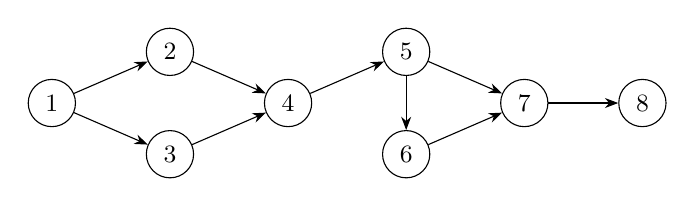
\begin{tikzpicture}[>=Stealth, every node/.style={circle, draw, fill=white, minimum size=6mm, inner sep=0.5pt, font=\small}]
  \node (n1) at (0,0) {1}; \node (n2) at (1.5,0.65) {2}; \node (n3) at (1.5,-0.65) {3};
  \node (n4) at (3,0) {4}; \node (n5) at (4.5,0.65) {5}; \node (n6) at (4.5,-0.65) {6};
  \node (n7) at (6,0) {7}; \node (n8) at (7.5,0) {8};
  \draw[->] (n1)--(n2); \draw[->] (n1)--(n3); \draw[->] (n2)--(n4); \draw[->] (n3)--(n4);
  \draw[->] (n4)--(n5); \draw[->] (n5)--(n6); \draw[->] (n5)--(n7); \draw[->] (n6)--(n7); \draw[->] (n7)--(n8);
\end{tikzpicture}
\end{center}
\opt{A. 12}\opt{B. 15}\opt{C. 18}\opt{D. 21}

\q{14.} 1 到 200 之间，不能被 2、3、7 中任何一个整除的整数共有（\qquad）个\\
\opt{A. 57}\opt{B. 58}\opt{C. 59}\opt{D. 60}
\begin{minipage}{\linewidth}
\q{15.} 已知如下 C++14 代码定义 Ackermann 函数：
\begin{codebox}\begin{lstlisting}
long long A(int m, long long n) {
    if (m == 0)
        return n + 1;
    if (n == 0)
        return A(m - 1, 1);
    return A(m - 1, A(m, n - 1));
}
\end{lstlisting}\end{codebox}
则二元组 \(\bigl(A(3,3),\,A(3,10^{18})\bmod 101\bigr)\) 的值为（\qquad）\\
\opt{A. \texttt{(61, 5)}}\opt{B. \texttt{(61, 8)}}
\opt{C. \texttt{(31, 5)}}\opt{D. \texttt{(31, 8)}}
\end{minipage}

\bigtitle{二、阅读程序（程序输入不超过数组或字符串定义的范围；判断题正确填√，错误填×；除特殊说明外，判断题 1.5 分，选择题 3 分，共计 40 分）}

\noindent（1）
\begin{codebox}\begin{lstlisting}
#include <bits/stdc++.h>
using namespace std;
const int N = 2e5 + 5;
int n, pi[N];
string s;

int main() {
    cin >> s;
    n = s.size();
    for (int i = 1; i < n; ++i) {
        int j = pi[i - 1];
        while (j && s[i] != s[j])
            j = pi[j - 1];
        if (s[i] == s[j])
            ++j;
        pi[i] = j;
    }
    int ans = 0;
    for (int len = n; len > 0; len = pi[len - 1])
        ans += len;
    cout << ans << '\n';
}
\end{lstlisting}\end{codebox}

\noindent\wdot\hspace{0.5em}判断题\\
\q{16.} 当输入字符串为 \texttt{ababa} 时，程序计算得到 \texttt{pi[4]=3}。（\qquad）\\
\opt{A. 正确}\opt{B. 错误}
\begin{minipage}{\linewidth}
\q{17.} 输入字符串为 \texttt{ababa}，程序执行第 19--20 行的累加循环后，输出为（\qquad）\\
\opt{A. 7}\opt{B. 8}\opt{C. 9}\opt{D. 10}
\end{minipage}
\q{18.} 输入字符串为 \texttt{bbba}。第 12 行的 \texttt{while} 保持不变时程序输出为 \texttt{X}；只将第 12 行的 \texttt{while} 改为 \texttt{if} 时程序输出为 \texttt{Y}。二元组 \texttt{(X,Y)} 为（\qquad）\\
\opt{A. \texttt{(4,5)}}\opt{B. \texttt{(5,4)}}
\opt{C. \texttt{(4,4)}}\opt{D. \texttt{(5,5)}}

\noindent\wdot\hspace{0.5em}单选题\\
\q{19.} 输入 \texttt{abacababacabab} 时，程序输出为（\qquad）\\
\opt{A. 16}\opt{B. 20}\opt{C. 24}\opt{D. 28}
\q{20.}（4 分）若输入字符串长度为 $n$，且字符比较、数组访问均视为 $O(1)$，则程序的最坏时间复杂度和空间复杂度分别为（\qquad）\\
\opt{A. 时间 $O(n^2)$，空间 $O(n)$}
\opt{B. 时间 $O(n)$，空间 $O(n)$}
\opt{C. 时间 $O(n\log n)$，空间 $O(1)$}
\opt{D. 时间 $O(n^2)$，空间 $O(1)$}

\noindent（2）
\begin{codebox}\begin{lstlisting}
#include <bits/stdc++.h>
using namespace std;
const int P = 998244353, M = 10;
int n, m, ban[105], f[2][1 << M];
vector<int> st;

int main() {
    cin >> n >> m;
    for (int i = 1; i <= n; ++i) {
        string s;
        cin >> s;
        for (int j = 0; j < m; ++j)
            if (s[j] == '#')
                ban[i] |= 1 << j;
    }
    for (int s = 0; s < (1 << m); ++s)
        if ((s & (s << 1)) == 0)
            st.emplace_back(s);
    f[0][0] = 1;
    for (int i = 1; i <= n; ++i) {
        int pre = i & 1, cur = pre ^ 1;
        int mask = pre ^ cur;
        pre ^= mask;
        cur ^= mask;

        memset(f[cur], 0, sizeof(f[cur]));
        for (auto &&s : st) {
            if (s & ban[i]) continue;
            for (auto &&t : st) {
                if (s & t)
                    continue;
                f[cur][s] += f[pre][t];
                if (f[cur][s] >= P)
                    f[cur][s] -= P;
            }
        }
    }
    int ans = 0;
    for (auto &&s : st) {
        ans += f[n & 1][s];
        if (ans >= P)
            ans -= P;
    }
    cout << ans << '\n';
}
\end{lstlisting}\end{codebox}

\noindent\wdot\hspace{0.5em}判断题\\
\q{21.} 当 \texttt{m=3} 时，经过第 16--18 行的状态枚举后，\texttt{st.size()} 的值为 5。（\qquad）\\
\opt{A. 正确}\opt{B. 错误}
\begin{minipage}{\linewidth}
\q{22.} 若某次枚举中 \texttt{s=101}、\texttt{t=001}，程序会执行 \texttt{continue}，不会把 \texttt{f[pre][t]} 加入当前结果。（\qquad）\\
\opt{A. 正确}\opt{B. 错误}
\end{minipage}
\q{23.}（2 分）输入为 \texttt{n=3,m=2}，三行均为 \texttt{..}。保留第 26 行与删除第 26 行后，程序输出的二元组（保留，删除）为（\qquad）\\
\opt{A. \texttt{(17,23)}}\opt{B. \texttt{(23,17)}}
\opt{C. \texttt{(17,17)}}\opt{D. \texttt{(23,23)}}

\noindent\wdot\hspace{0.5em}单选题\\
\q{24.} 记 \(V=\texttt{st.size()}\)，则程序的时间复杂度为（\qquad）\\
\opt{A. \(O(nV)\)}\opt{B. \(O(nV^2+2^m)\)}\opt{C. \(O(n2^{2m})\)}\opt{D. \(O(n^2V)\)}
\q{25.} 输入为 \texttt{n=2,m=3}，两行均为 \texttt{...} 时，程序输出为（\qquad）\\
\opt{A. 15}\opt{B. 16}\opt{C. 17}\opt{D. 18}
\q{26.} 输入为 \texttt{n=3,m=2}，三行均为 \texttt{..}。保留第 23--24 行与删除这两行后，程序输出的二元组（保留，删除）为（\qquad）\\
\opt{A. \texttt{(17,0)}}\opt{B. \texttt{(0,17)}}
\opt{C. \texttt{(17,17)}}\opt{D. \texttt{(0,0)}}

\noindent（3）
\begin{codebox}\begin{lstlisting}
#include <bits/stdc++.h>
using namespace std;
using ll = long long;
const ll P = 1000000007;
const int N = 2e5 + 5;
int n, q;
ll a[N];
struct Node {
    ll sum, mul, add;
} tr[N << 2];

void build(int p, int l, int r) {
    tr[p].mul = 1;
    if (l == r) {
        tr[p].sum = a[l] % P;
        return;
    }
    int m = (l + r) >> 1;
    build(p << 1, l, m);
    build(p << 1 | 1, m + 1, r);
    tr[p].sum = (tr[p << 1].sum + tr[p << 1 | 1].sum) % P;
}
void apply(int p, int l, int r, ll k, ll b) {
    tr[p].sum = (tr[p].sum * k + (r - l + 1) * b) % P;
    tr[p].mul = tr[p].mul * k % P;
    tr[p].add = (tr[p].add * k + b) % P;
}
void push(int p, int l, int r) {
    if (l == r)
        return;
    int m = (l + r) >> 1;
    apply(p << 1, l, m, tr[p].mul, tr[p].add);
    apply(p << 1 | 1, m + 1, r, tr[p].mul, tr[p].add);
    std::exchange(tr[p].mul, 1);
    std::exchange(tr[p].add, 0);
}
void upd(int p, int l, int r, int ql, int qr, ll k, ll b) {
    if (ql <= l && r <= qr) {
        apply(p, l, r, k, b);
        return;
    }
    push(p, l, r);
    int m = (l + r) >> 1;
    if (ql <= m)
        upd(p << 1, l, m, ql, qr, k, b);
    if (qr > m)
        upd(p << 1 | 1, m + 1, r, ql, qr, k, b);
    tr[p].sum = (tr[p << 1].sum + tr[p << 1 | 1].sum) % P;
}
ll qry(int p, int l, int r, int ql, int qr) {
    if (ql <= l && r <= qr)
        return tr[p].sum;
    push(p, l, r);
    int m = (l + r) >> 1;
    ll s = 0;
    if (ql <= m)
        s = (s + qry(p << 1, l, m, ql, qr)) % P;
    if (qr > m)
        s = (s + qry(p << 1 | 1, m + 1, r, ql, qr)) % P;
    return s;
}
int main() {
    cin >> n >> q;
    for (int i = 1; i <= n; ++i)
        cin >> a[i];
    build(1, 1, n);
    while (q--) {
        int op, l, r;
        cin >> op >> l >> r;
        if (!(op ^ 1)) {
            ll k, b;
            cin >> k >> b;
            upd(1, 1, n, l, r, k, b);
        } else
            cout << qry(1, 1, n, l, r) << '\n';
    }
}
\end{lstlisting}\end{codebox}

\noindent\wdot\hspace{0.5em}判断题\\
\begin{minipage}{\linewidth}
\q{27.} 在执行一次 \texttt{upd} 时，如果当前结点区间完全包含在更新区间内，程序会执行第 38--40 行：调用一次 \texttt{apply} 后直接返回，不再访问该结点的子结点。（\qquad）\\
\opt{A. 正确}\opt{B. 错误}
\end{minipage}
\q{28.} 若把第 34--35 行中 \texttt{push} 末尾的 \texttt{tr[p].add} 重置语句删去，程序对所有输入的输出仍然不变。（\qquad）\\
\opt{A. 正确}\opt{B. 错误}
\q{29.} 程序的时间复杂度为 \(O((n+q)\log n)\)。（\qquad）\\
\opt{A. 正确}\opt{B. 错误}

\noindent\wdot\hspace{0.5em}单选题\\
\q{30.} 设当前结点 \texttt{p} 表示区间 \([l,r]\)，执行第 39 行调用的 \texttt{apply(p,l,r,k,b)} 后，\texttt{tr[p].sum} 的新值为（\qquad）\\
\opt{A. \texttt{(tr[p].sum*k+b) \% P}}
\opt{B. \texttt{(tr[p].sum*k+(r-l+1)*b) \% P}}
\opt{C. \texttt{((tr[p].sum+b)*k) \% P}}
\opt{D. \texttt{((r-l+1)*(tr[p].sum*k+b)) \% P}}
\q{31.} 关于第 28--36 行的函数 \texttt{push}，下列修改中不会改变程序输出的是（\qquad）\\
\opt{A. 交换左、右子结点调用 \texttt{apply} 的先后顺序}
\opt{B. 在调用两个子结点的 \texttt{apply} 前，先把 \texttt{tr[p].add} 置为 0}
\opt{C. 把两个 \texttt{apply} 调用中的参数 \texttt{b} 都改为 0}
\opt{D. 删除右子结点的 \texttt{apply} 调用，但保留左子结点的调用}
\q{32.}（4 分）初始数组为 \texttt{2 1 3 5 4 6}，依次执行 \texttt{1 2 6 2 1}、\texttt{1 1 4 3 2}、\texttt{1 3 5 1 4}、\texttt{2 2 6}，最后一次操作输出为（\qquad）\\
\opt{A. 99}\opt{B. 103}\opt{C. 105}\opt{D. 107}
\clearpage
\bigtitle{三、完善程序（单选题，每小题 3 分，共计 30 分）}

\noindent（1）（序列）给定一个长度为 \texttt{n}、只含字符 \texttt{R,G,Y} 的字符串。每次可以交换两个相邻字符。求使相邻字符均不同所需的最少交换次数；若无法做到，输出 \texttt{-1}。\texttt{1 <= n <= 400}。

\begin{codebox}\begin{lstlisting}
#include <bits/stdc++.h>
using namespace std;
const int N = 405, INF = 1e9;
int n, cnt[3], pos[3][N], pre[3][N];
int f[2][N][N][4];
string s;
int main() {
    cin >> n >> s;
    for (int i = 1; i <= n; ++i) {
        int c;
        if (s[i - 1] == 'R')
            c = 0;
        else if (s[i - 1] == 'G')
            c = 1;
        else
            c = 2;
        for (int t = 0; t < 3; ++t)
            pre[t][i] = |@\blank{①}@|;
        pos[c][++cnt[c]] = i;
        ++pre[c][i];
    }
    memset(f, 0x3f, sizeof(f));
    f[0][0][0][3] = |@\blank{②}@|;
    for (int len = 0; len < n; ++len) {
        int cur = len & 1, nxt = cur ^ 1;
        memset(f[nxt], 0x3f, sizeof(f[nxt]));
        for (int r = 0; r <= cnt[0]; ++r)
            for (int g = 0; g <= cnt[1]; ++g) {
                int y = |@\blank{③}@|;
                if (y < 0 || y > cnt[2])
                    continue;
                int used[3] = {r, g, y};
                for (int last = 0; last < 4; ++last) {
                    int val = f[cur][r][g][last];
                    if (val >= INF)
                        continue;
                    for (int c = 0; c < 3; ++c) {
                        if (|@\blank{④}@|)
                            continue;
                        int x = pos[c][used[c] + 1];
                        int w = x - len - 1;
                        for (int t = 0; t < 3; ++t)
                            w += max(0,used[t]-pre[t][x]);
                        int nr = r, ng = g;
                        if (c == 0)
                            ++nr;
                        if (c == 1)
                            ++ng;
                        int nv = |@\blank{⑤}@|;
                        f[nxt][nr][ng][c] =
                            min(f[nxt][nr][ng][c], nv);
                    }
                }
            }
    }
    int ans = INF, z = n & 1;
    for (int c = 0; c < 3; ++c) {
        int v = f[z][cnt[0]][cnt[1]][c];
        ans = min(ans, v);
    }
    cout << (ans >= INF ? -1 : ans) << '\n';
}
\end{lstlisting}\end{codebox}

\q{33.} 第18行①处应填（\qquad）\\
\optw{A. \texttt{pre[t][i-1]}}{B. \texttt{pre[t][i] + 1}}
\optw{C. \texttt{pre[t][i-1] + (t == c)}}{D. \texttt{pre[c][i-1]}}
\q{34.} 第23行②处应填（\qquad）\\
\optw{A. \texttt{INF}}{B. \texttt{0}}
\optw{C. \texttt{1}}{D. \texttt{len}}
\q{35.} 第29行③处应填（\qquad）\\
\optw{A. \texttt{len-r-g}}{B. \texttt{r+g-len}}
\optw{C. \texttt{n-r-g}}{D. \texttt{cnt[2]-r-g}}
\q{36.} 第38行④处应填（\qquad）\\
\optw{A. \texttt{c == last || used[c] == cnt[c]}}{B. \texttt{c != last \&\& used[c] < cnt[c]}}
\optw{C. \texttt{c == last \&\& used[c] == cnt[c]}}{D. \texttt{c != last || used[c] < cnt[c]}}
\begin{samepage}
\q{37.} 第49行⑤处应填（\qquad）\\
\optw{A. \texttt{val}}{B. \texttt{w}}
\optw{C. \texttt{val + w}}{D. \texttt{val + len - w}}
\end{samepage}

\noindent（2）（盒子）有 \texttt{n} 个体积互不相同的盒子和 \texttt{k} 个物品。每个盒子中恰放一个物品或一个体积更小的盒子；把体积为 \(x\) 的盒子放入体积为 \(y\) 的盒子需要 \(y-x\) 单位缓冲材料。所有盒子均须使用。先求所需缓冲材料的最小总量；随后有 \texttt{q} 次删除，每次永久删除一个指定盒子并再次求答案。保证始终至少剩下 \texttt{k} 个盒子。\texttt{1 <= n <= 2*10\string^5}。

\begin{codebox}\begin{lstlisting}
#include <bits/stdc++.h>
using namespace std;
using ll = long long;
const int N = 2e5 + 5;
int n, k, q, need;
ll c[N], ans;
set<ll> box;
multiset<ll> lo, hi;

void fix() {
    while ((int)lo.size() > need) {
        auto it = |@\blank{①}@|;
        ans -= *it;
        hi.insert(*it);
        lo.erase(it);
    }
    while ((int)lo.size() < need) {
        auto it = hi.begin();
        ans += *it;
        lo.insert(*it);
        hi.erase(it);
    }
    while (!lo.empty() && !hi.empty()) {
        auto x = prev(lo.end()), y = hi.begin();
        if (|@\blank{②}@|)
            break;
        ll vx = *x, vy = *y;
        ans += |@\blank{③}@|;
        lo.erase(x);
        hi.erase(y);
        lo.insert(vy);
        hi.insert(vx);
    }
}
void add_gap(ll x) {
    lo.insert(x);
    ans += x;
}
void del_gap(ll x) {
    auto it = lo.find(x);
    if (it != lo.end()) {
        ans -= x;
        lo.erase(it);
    } else
        hi.erase(hi.find(x));
}
int main() {
    cin >> n >> k;
    for (int i = 1; i <= n; ++i) {
        cin >> c[i];
        box.insert(c[i]);
    }
    if (box.size() > 1) {
        auto x = box.begin(), y = next(x);
        for (; y != box.end(); ++x, ++y)
            add_gap(*y - *x);
    }
    need = |@\blank{④}@|;
    fix();
    cout << ans << '\n';
    cin >> q;
    while (q--) {
        int d;
        cin >> d;
        ll v = c[d], l = 0, r = 0;
        auto it = box.find(v);
        auto rt = next(it);
        bool hl = it != box.begin();
        bool hr = rt != box.end();
        if (hl) {
            l = *prev(it);
            del_gap(v - l);
        }
        if (hr) {
            r = *rt;
            del_gap(r - v);
        }
        box.erase(it);
        --need;
        if (hl && hr)
            add_gap(|@\blank{⑤}@|);
        fix();
        cout << ans << '\n';
    }
}
\end{lstlisting}\end{codebox}

\q{38.} 第12行①处应填（\qquad）\\
\optw{A. \texttt{lo.begin()}}{B. \texttt{prev(lo.end())}}
\optw{C. \texttt{hi.begin()}}{D. \texttt{prev(hi.end())}}
\q{39.} 第26行②处应填（\qquad）\\
\optw{A. \texttt{*x < *y}}{B. \texttt{*x <= *y}}
\optw{C. \texttt{*x > *y}}{D. \texttt{*x >= *y}}
\q{40.} 第28行③处应填（\qquad）\\
\optw{A. \texttt{vx - vy}}{B. \texttt{vy - vx}}
\optw{C. \texttt{vx + vy}}{D. \texttt{-vx}}
\q{41.} 第58行④处应填（\qquad）\\
\optw{A. \texttt{n - k}}{B. \texttt{k - 1}}
\optw{C. \texttt{n - 1}}{D. \texttt{k}}
\q{42.} 第81行⑤处应填（\qquad）\\
\optw{A. \texttt{v - l}}{B. \texttt{r - v}}
\optw{C. \texttt{r - l}}{D. \texttt{r + l - v}}

\end{document}
